\documentclass[a4paper]{article}
\usepackage{graphicx}
\usepackage{amsmath}
\usepackage{amsmath}
\usepackage[section]{placeins}
\usepackage{geometry}
 \geometry{
 a4paper,
 total={150mm,257mm},
 top=20mm,
 }
\begin{document}

\begin{figure}
	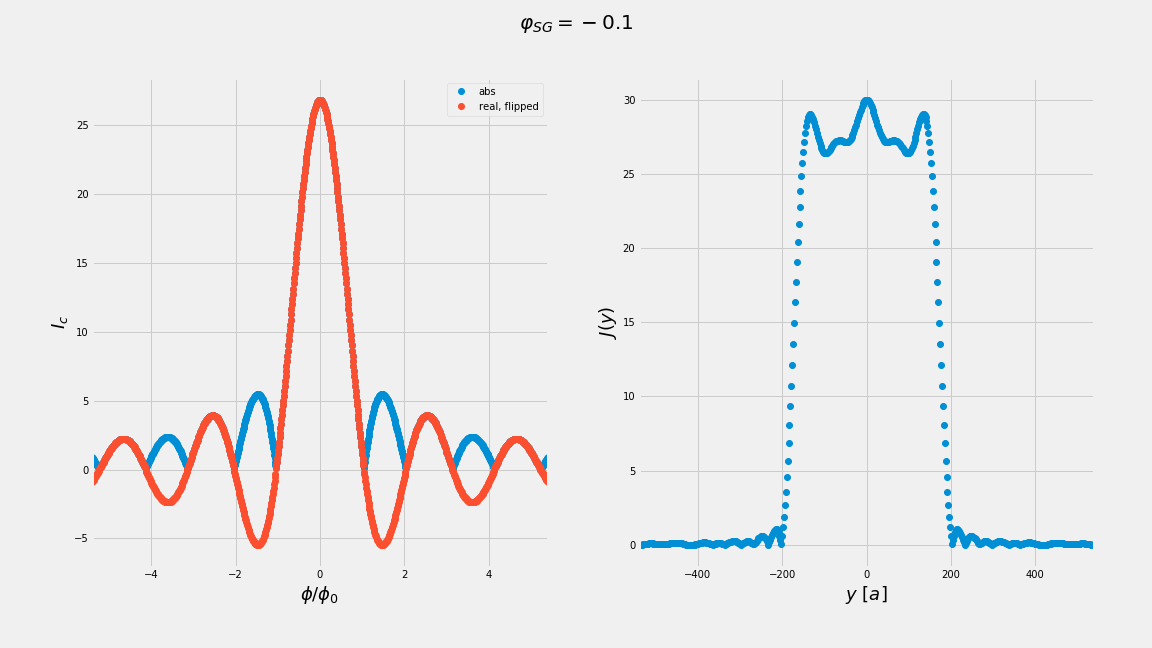
\includegraphics[width=0.9\textwidth]{figs/wg32/current_and_density_01}
	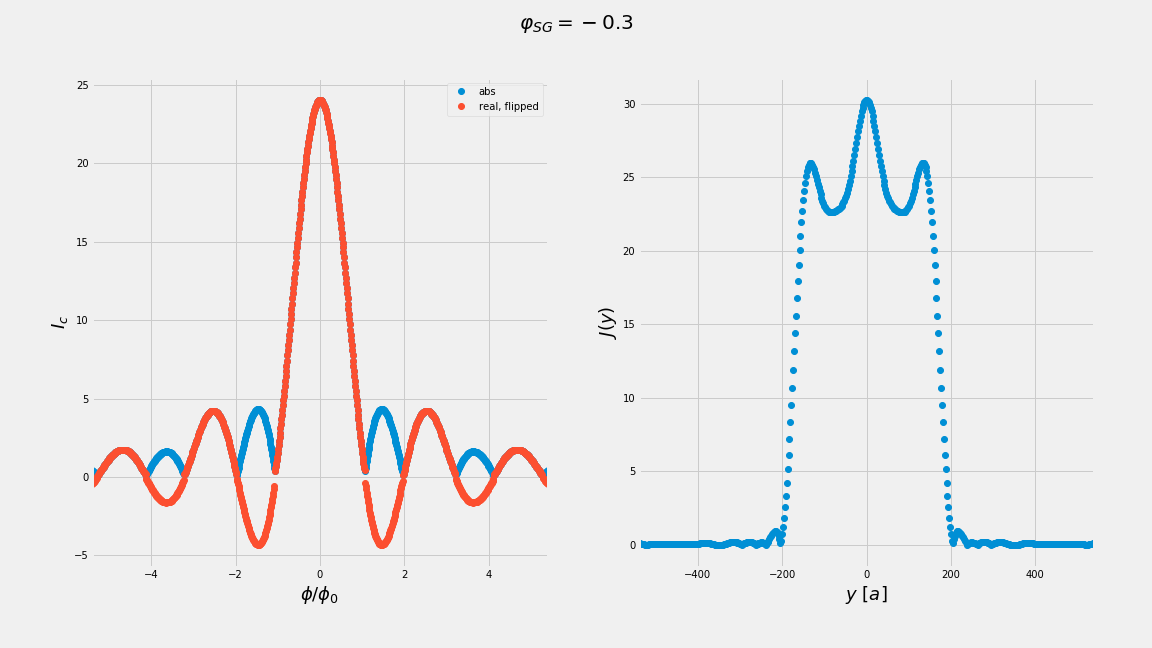
\includegraphics[width=0.9\textwidth]{figs/wg32/current_and_density_03}
	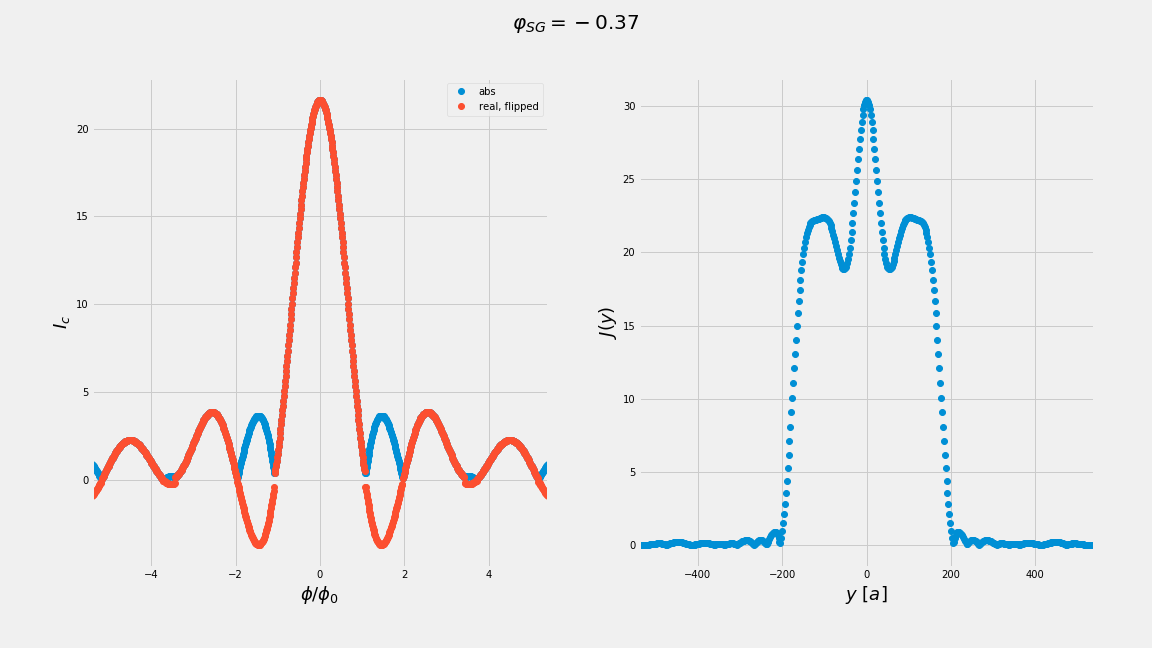
\includegraphics[width=0.9\textwidth]{figs/wg32/current_and_density_037}
\end{figure}
\begin{figure}
	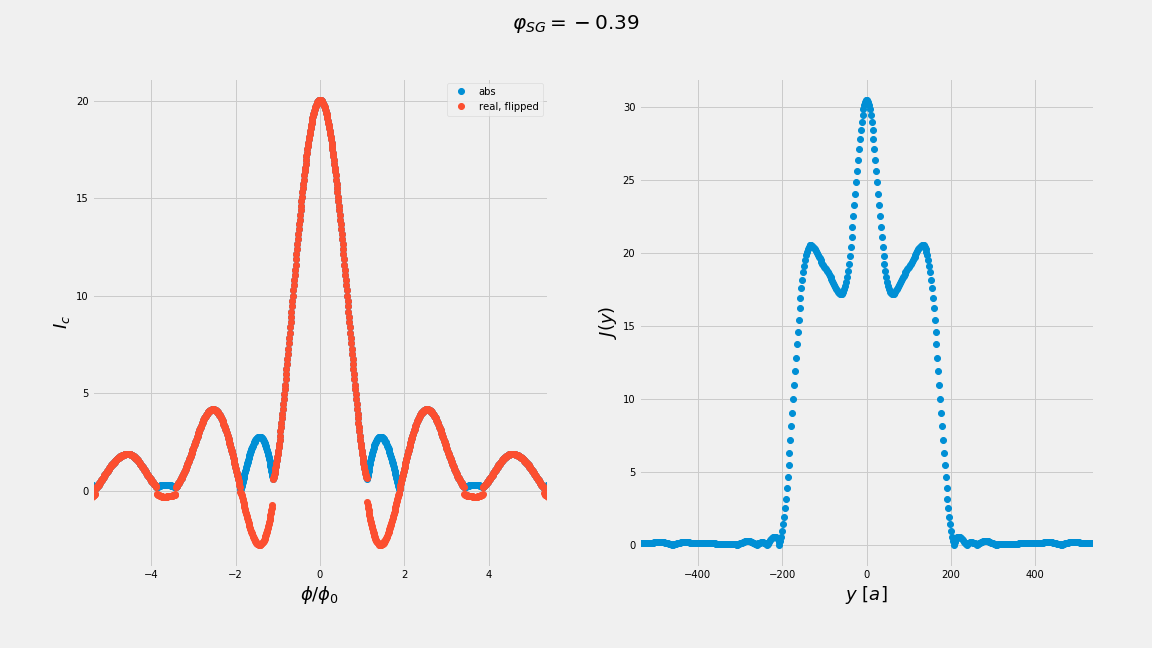
\includegraphics[width=0.9\textwidth]{figs/wg32/current_and_density_039}
	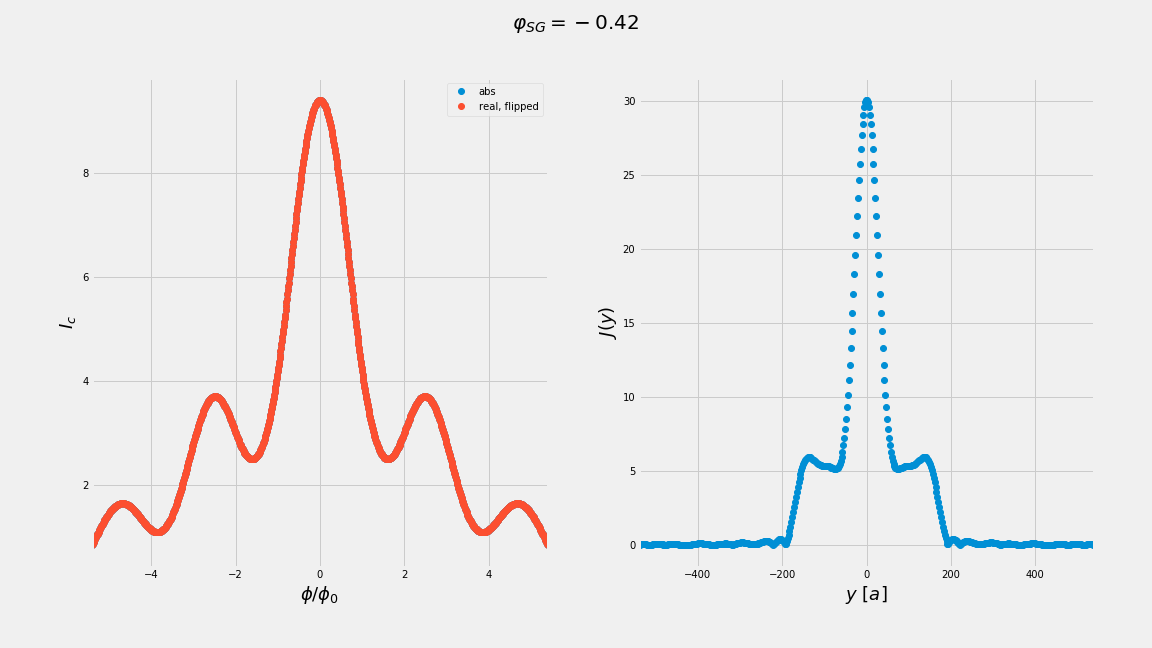
\includegraphics[width=0.9\textwidth]{figs/wg32/current_and_density_042}
	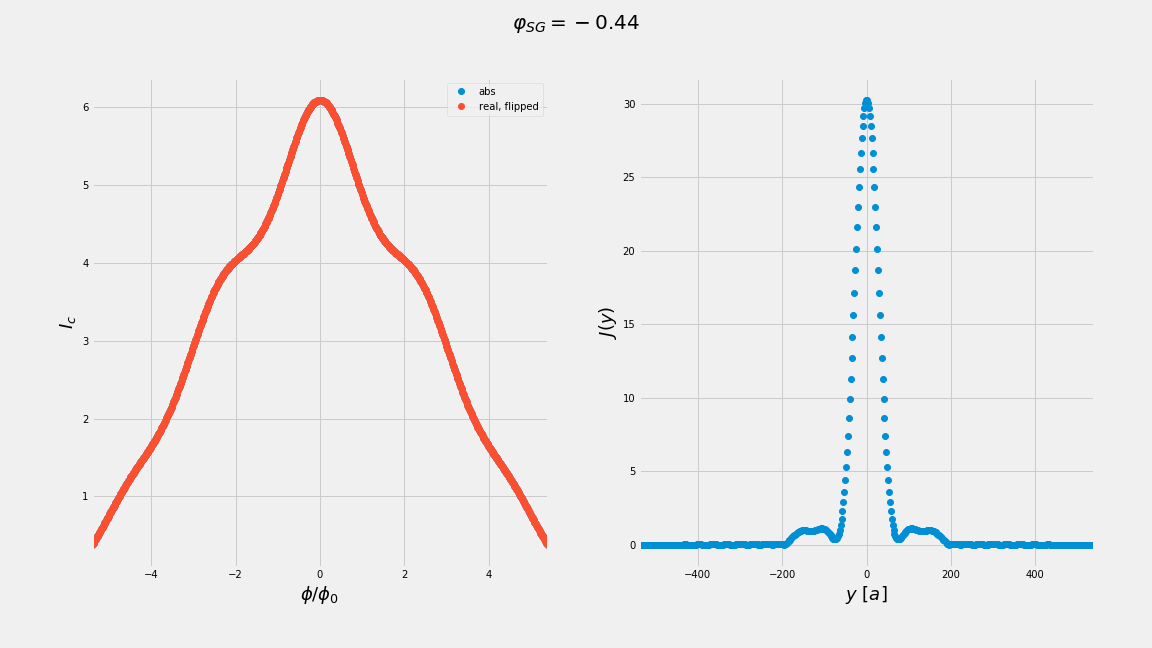
\includegraphics[width=0.9\textwidth]{figs/wg32/current_and_density_044}
\end{figure}
\begin{figure}
	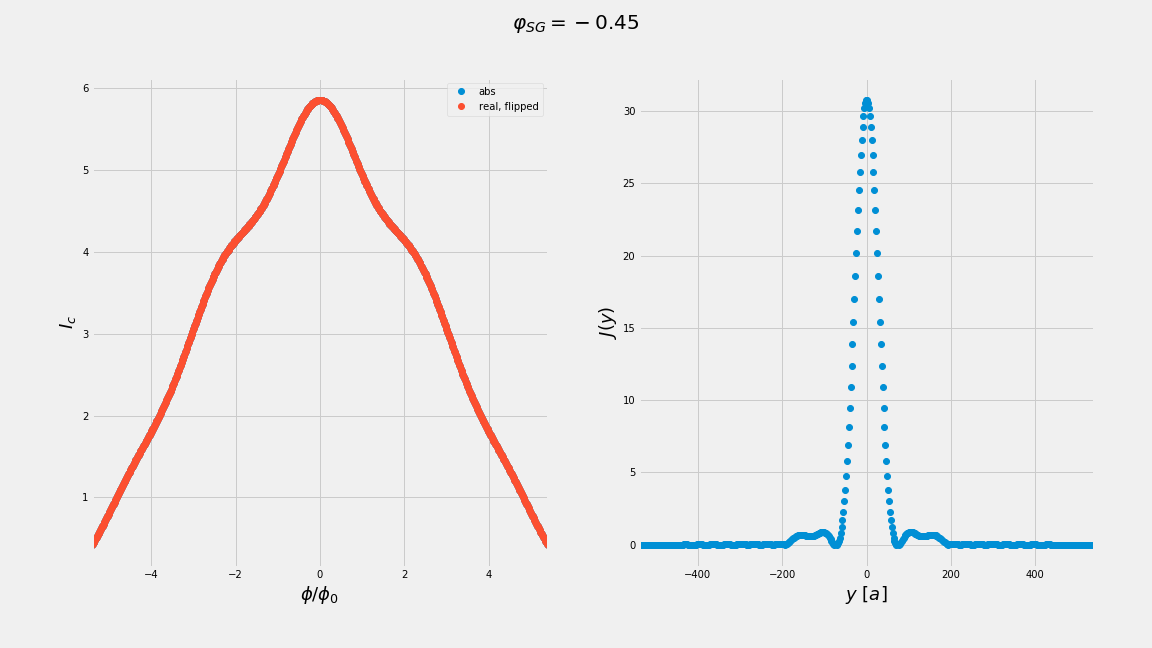
\includegraphics[width=0.9\textwidth]{figs/wg32/current_and_density_045}
	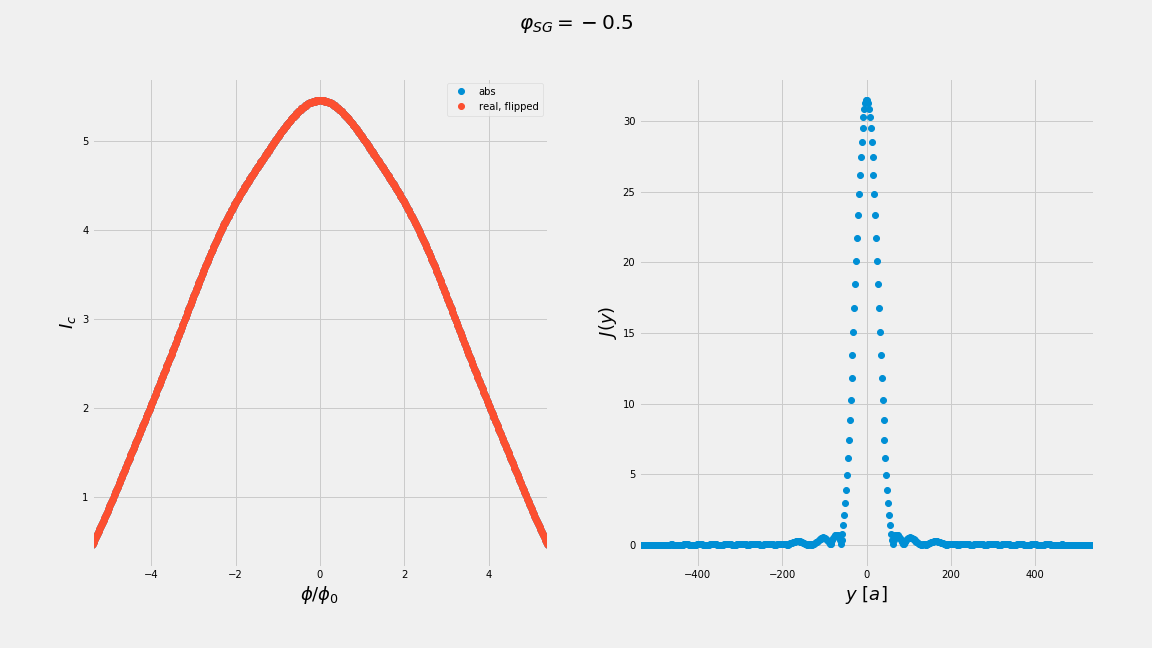
\includegraphics[width=0.9\textwidth]{figs/wg32/current_and_density_05}
	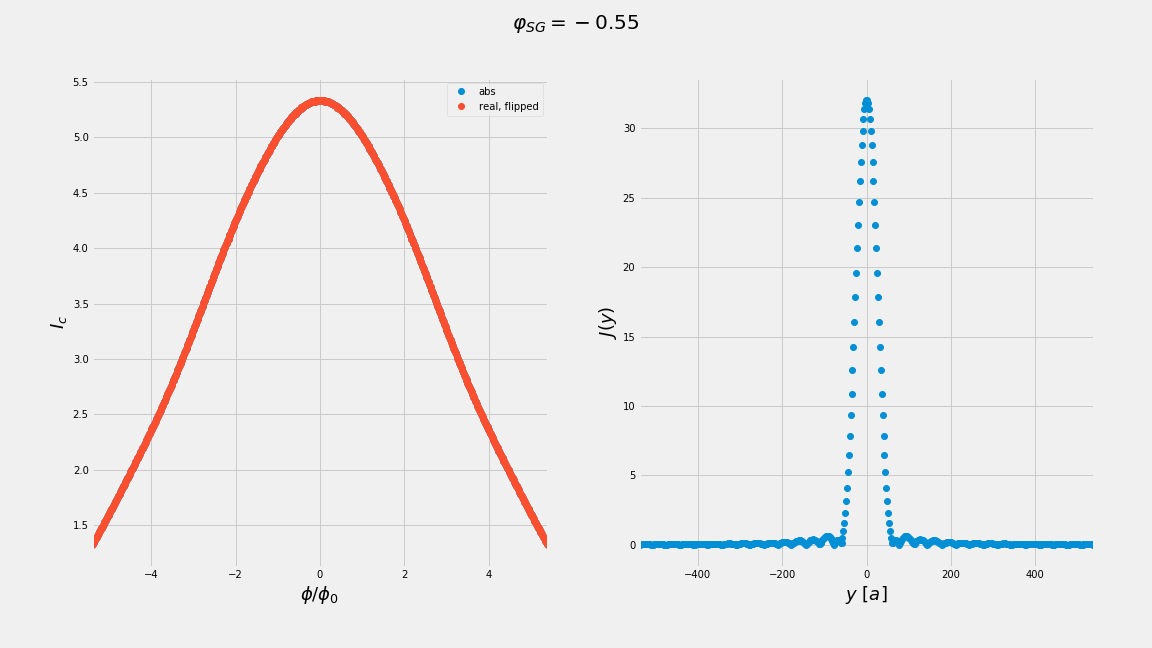
\includegraphics[width=0.9\textwidth]{figs/wg32/current_and_density_055}
\end{figure}

\end{document}
